%!TEX root =  bgo-cam-ready.tex
% please do not delete or change the first line (needed by Csaba's editor)

\textit{Notation:} Capital letters will denote random variables.
For $i\le j$ positive integers,
 we use the notation $a_{i:j}$ to denote
 the sequence $(a_i,a_{i+1}, \dots, a_{j})$.

 We let $\| \cdot \|$ denote some norm on $\R^d$, whose dual is denoted by $\dnorm{\cdot}$. 
 Let $\K \subset \R^d$ be a non-empty closed convex  set. 
 Given the function $f:\K \to \R$ which is differentiable%
\footnote{Here we assume the differentiablity for simplicity of definition, actually it is easy to generalize to non-differentiable functions by using sub-gradient.} 
  in $\K^\circ$,%
  \footnote{For $A\subset \mathbb{R}^d$, $A^\circ$ denotes the interior of $A$.}
 $f$ is said to be $\mu$-strongly convex w.r.t.\  $\| \cdot \|$  ($\mu\ge 0$) if
 $\tfrac{\mu}{2} \|x-y\|^2 \le \mathcal{D}_f(x,y)\doteq f(x)-f(y)-\ip{\nabla f(y),x-y}$, for all $x \in \K \,, y \in \K^\circ$.
Similarly, $f$ is $\mu$-strongly convex w.r.t.\  a \emph{function} $\cR$
	if $\tfrac{\mu}{2}\DR(x,y)\le\mathcal{D}_f(x,y)$ for all $x \in \K \,, y \in \K^\circ$, where $\cK^\circ\subseteq \dom(\mathcal{R})$ and $\mathcal{R}$ is differentiable over $\K^\circ$.
 A function $f$ is $L$-smooth w.r.t.\  $\| \cdot \| $ for some $L>0$ if
 %$f(x) \le f(y) + \ip{\nabla f(y), y-x} +
$D_f(x,y) \le \tfrac{L}{2} \|x-y\|^2$, for all $x \in \K \,, y \in \K^\circ$.
 This latter condition is equivalent to that $\nabla f$ is $L$-Lipschitz, that is, 
 $\norm{\nabla f(x) - \nabla f(y)}_* \le L \norm{x-y}$ \citep[Theorem~2.1.5]{nesterov2004introductory}.
% \todoc{Add citation}
 We let $\F_{L,\mu, \cR}(\K)$ denote the class of functions that are $\mu$-strongly convex w.r.t. $\cR$ and $L$-smooth w.r.t. some norm $\norm{\cdot}$ on the set $\K$ (typically, we will assume that $\cR$ is also strongly convex w.r.t. $\norm{\cdot}$).
We also let $\F_{L,\mu}(\K)$ be $\F_{L,\mu,\cR}(\cK)$ with $\cR(\cdot) = \frac12 \norm{\cdot}_2^2$.
Then, the set of convex and $L$-smooth functions is  $\F_{L,0}(\K)$.
 %Furthermore, let $\F_{L,\mu,\cR}(\K)$ denote the set of functions that are  $L$-smooth and $\mu$-strongly convex w.r.t.\  $\cR$. \todoc{Are these $L$-smooth w.r.t. $\cR$? This is a bit confusing.}
% We let $\normal(0, I)$ denote the standard normal distribution in $d$-dimensions. 
% \todoc{I am pretty sure $\normal(0, I)$ is not used in the main text, hence commenting it out. We will need to define it for the full version!!!}

\begin{figure}
\begin{center}
\vspace{-0.1cm}
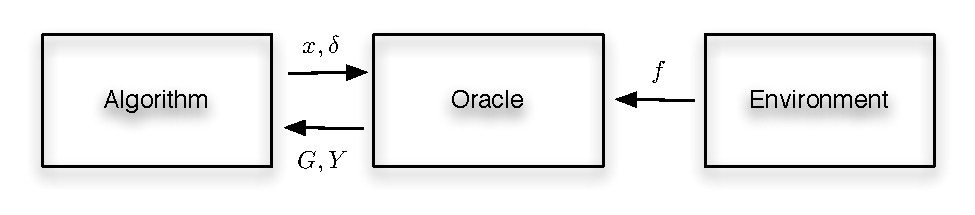
\includegraphics[width=0.45\textwidth]{../figs/oracle}
\end{center}
\vspace{-0.6cm}
\caption{The Interaction of the algorithms with the gradient estimation oracle and the environment. For more information, see the text. \vspace{-0.3cm}}
\label{fig:oracle}
\end{figure}

In this paper, we consider convex optimization in a novel setting, both for stochastic as well as online BCO.
%More specifically, we consider both an online learning setting and an optimization setting.
In the online BCO setting, the environment chooses a sequence of loss functions $f_1,\dots,f_n$ belonging to a set $\cF$ of convex functions over a common, non-empty convex closed domain $\cK\subset \R^d$.
In the stochastic BCO setting, a single fixed loss function $f\in \cF$ is chosen.
An algorithm chooses a sequence of points $X_1,\dots,X_n\in \cK$ in a serial fashion.
The novelty of our setting is that the algorithm, upon selecting point $X_t$, receives
a noisy and potentially biased estimate $G_t\in \R^d$
of the gradient of the loss function $f$
(more generally, an estimate of a subgradient of $f$, in case $f$ is not differentiable at $X_t$).
To control the bias and the variance, the algorithm can choose a \emph{tolerance parameter} $\delta_t>0$
(in particular, we allow the algorithms to choose the tolerance parameter sequentially).
A smaller $\delta_t$ results in a smaller ``bias'' (for the precise meaning of bias, we will consider two definitions below), while typically with a smaller $\delta_t$, the ``variance'' of the gradient estimate increases.
Notice that in the online BCO setting, the algorithm suffers the loss $f_t(Y_t)$ in round $t$, where $Y_t\in \cK$\footnote{For simplicity, in some cases we allow $f$ to be defined outside of $\K$ and allow $Y_t$ to be in a small vicinity of $\K$.} is guaranteed to be in the $\delta_t$-vicinity of $X_t$.
%While this point is not relevant in the optimization setting, in the online learning setting,
The goal in the online BCO setting is to keep the expected \emph{regret},
	$R_n =\EE{ \sum_{t=1}^n f_t(Y_t)} - \inf_{x\in \cK} \sum_{t=1}^n f_t(x)$,
small.
In the stochastic BCO setting, the algorithm is also required to select a point $\hat{X}_n\in \cK$ once
the $n$th round is over (in both settings, $n$ is given to the algorithms)
and the algorithm's performance is quantified using the \emph{optimization error},
$\Delta_n = \EE{f(\hat{X}_n)} - \inf_{x\in \cK} f(x) $.

The main novelty of the model is that the information flow between the algorithm and the environment (holding $f$, or $f_{1:n}$) is mediated by a gradient estimation oracle. As we shall see, numerous existing approaches to online learning and optimization based on noisy pointwise information fit in this framework.

We will use two classes of oracles. In both cases, the oracles are specified by
two functions $c_1,c_2:[0,\infty)\to [0,\infty)$, which will be assumed to be continuous,
monotonously increasing (resp., decreasing) with
$\lim_{\delta\to  0} c_1(\delta)=0$ and $\lim_{\delta\to 0} c_2(\delta)=+\infty$.
Typical choices for $c_1,c_2$ are $c_1(\delta) = C_1 \delta^p$, $c_2(\delta) = C_2\delta^{-q}$ with $p,q>0$.
Our type-I oracles are defined as follows:
%The relationship between these oracles will be studied in \cref{sec:orrel}.
%\todoc{$Y$ should be removed completely, and added only when online learning is considered.}
\vspace{-0.2cm}
\begin{definition}[$(c_1,c_2)$ type-I  oracle]
\label{def:oracle1}
We say that $\gamma$ is a  $(c_1,c_2)$ type-I oracle for $\cF$, if for any function $f\in \cF$,
$x\in \cK,0<\delta\le 1$, $\gamma$ returns $G\in \R^d$ and  $Y\in \cK$ random elements such that
$\norm{x-Y}\le \delta$ almost surely (a.s.),
\vspace{-0.2cm}
\begin{enumerate}
%\item $\norm{x-Y}\le \delta$ almost surely (a.s.);
\item $\norm{ \EE{G}  - \nabla f(x)  }_* \le c_1(\delta) $ (bias); and
\item $\EE{\norm{ G -  \EE{G} }_*^2} \le c_2(\delta)$.
\end{enumerate}
\vspace{-0.1cm}
\end{definition}
The upper bound on $\delta$ is arbitrary: by changing the norm, any other value can also be accommodated. Also, the upper bound only matters when $\K$ is bounded and the functions in $\cF$ are defined only in a small vicinity of $\K$.
\todoc[inline]{For precision, we should take conditional expectations given the past in the above definitions.}

The second type of oracles considered is as follows: \todoa{Here we could distinguish between the class of $f$ and $\tf$: we basically do not need to assume anything about $f$ as long as $\tf$ belongs to a nice enough family.}
\begin{definition}[$(c_1,c_2)$ type-II  oracle]
\label{def:oracle2}
We say that $\gamma$ is a  $(c_1,c_2)$ type-II oracle for $\cF$, if for any function $f\in \cF$,
$x\in \cK,0<\delta\le 1$, $\gamma$ returns $G\in \R^d$ and  $Y\in \cK$ random elements such that $\norm{x-Y}\le \delta$ a.s.,
\vspace{-0.2cm}
\begin{enumerate}
%\item $\norm{x-Y}\le \delta$ a.s.;
\item There exists $\tilde{f} \in \cF$ such that
$\norm{\tilde{f}- f}_\infty \le c_1(\delta)$  and
$\EE{G}  = \nabla \tilde{f}(x)$ (bias); and
\item $\EE{\norm{ G -  \EE{G} }_*^2} \le c_2(\delta)$ (variance).
\end{enumerate}
\vspace{-0.1cm}
\end{definition}
%An alternative to the bias condition for type-II oracles, which will also be considered later, is to replace the condition $\norm{\tilde{f}-f}_\infty \le c_1(\delta)$ with%
%\footnote{
%This definition requires the function $f$ to be differentiable. When the functions in $f$ are not differentiable, it is possible
%to modify the definitions to use subgradients. For simplicity, we will not consider this here.
%}
%\begin{align}
%\label{eq:oracle2alt}
%\norm{\nabla \tilde{f}- \nabla f}_* \le c_1(\delta)
%\end{align}
%We call the resulting oracles type-IIb.
%
Note that our definition allows the same oracle $\gamma$ to respond to the same inputs $(x,\delta,f)$ with a differently constructed pair (e.g., to have memory),
though most often the oracles constructed in practice
will map the triples $(x,\delta,f)$ to a gradient estimate-point pair using a fixed stochastic mapping.%
\footnote{For oracles with memory, in the definition the expectation should be replaced with
an expectation that is conditioned on the past.}
% \todoc{In fact, I am not sure which definition we should use. So things might change here.}
Examples will be discussed in  \cref{sec:sbco}. We also note that for type-II oracles we only need properties of the function class which the surrogate function $\tilde{f}$ belongs to, the assumption $f \in \F$ is only included to simplify the definition (e.g., our methods work for non-convex functions $f$ for which a suitable convex surrogate and the associated oracle exists).
We will denote the set of type-I (type-II) oracles satisfying the $(c_1,c_2)$-requirements given a function $f\in \cF$ by $\Gamma_1(f,c_1,c_2)$ (resp., $\Gamma_2(f,c_1,c_2)$).



Here, we will study the minimax regret in the online convex optimization setting, 
 while we study the minimax error in the stochastic convex optimization setting (sometimes, also called as the ``simple regret'').
Both are defined with respect to a class of loss functions $\cF$, and the bias/variance control functions $c_1,c_2$.
The \emph{wost case regret} of algorithm $\A$ interacting with $(c_1,c_2)$ type-I oracles for the function class $\F$ is

\begin{align*}
%\MoveEqLeft
R_{\F,n}^\cA(c_1,c_2)
&=  \sup_{f_{1:n}\in \cF^n}
	\sup_{\substack{\gamma_t \in \Gamma_1(f_t,c_1,c_2)\\1\le t \le n
	}} R_n^{\cA}(f_{1:n},\gamma_{1:n})
%\label{eq:minimaxregdef}
%\\
%\MoveEqLeft
%= \inf_{\cA} \sup_{f_{1:n}\in \cF}
%	\sup_{\substack{\gamma_t \in \Gamma_1(f_t,c_1,c_2)\\1\le t \le n}}
%\EE{ \sum_{t=1}^n f_t(Y_t) }
%%%%%%& \qquad \qquad \qquad \qquad \qquad
%-\inf_{x\in \cK} \sum_{t=1}^n f_t(x)\,,\\
\end{align*}
where $R_n^{\cA}(f_{1:n},\gamma_{1:n})$ denotes the expected regret of $\cA$ (against $f_{1:n},\gamma_{1:n}$), and
the \emph{minimax expected regret} for $(\cF,c_1,c_2)$ with type-I oracles is defined as
\[
R_{\F,n}^*(c_1,c_2) = \inf_{\cA} R_{\F,n}^\cA(c_1,c_2),
\]
where $\cA$ ranges through all algorithms that interact with the loss sequence  $f_{1:n}= (f_1,\dots,f_n)$
through the oracles $\gamma_{1:n}$ (in round $t$, oracle $\gamma_t$ is used).
The minimax regret for type-II oracles is defined analogously.
% (in what follows we only define these quantities for type-I oracles, as the extension \todoc{Is extension the right word?}
% to type-II oracles is immediate).


In the stochastic BCO setting, the \emph{worst case error} is defined through
\begin{align}
\label{eq:minimaxerrdef}
\Delta_{\F,n}^\cA(c_1,c_2)
= \sup_{f \in \cF} \sup_{\gamma\in \Gamma_1(f,c_1,c_2)}  \Delta_n^{\cA}(f,\gamma)\,, %(f,\gamma)\,,
% \EE{ f(\hat{X}_n) } - \inf_{x\in \cK}  f(x)\,,
\end{align}
where $\Delta_n^{\cA}(f,\gamma)$ is the optimization error that $\cA$ suffers
after $n$ rounds of interaction with $f$ through (a single) $\gamma$ as described earlier, and the \emph{minimax error}
is defined as
\[
\Delta_{\F,n}^*(c_1,c_2) =  \inf_{\cA} \Delta_{\F,n}^\cA(c_1,c_2),
\]
where, again, $\cA$ ranges through all algorithms that interact with $f$ through an oracle.
The minimax error for type-II oracles is defined analogously.

When the set $\K$ is bounded and the function set $\F$ is invariant to linear shifts, every $(c_1,c_2)$ type-I oracle is also an $(R c_1,c_2)$ type-II oracle,
where $R = \sup_{x\in \K} \norm{x}$: simply consider $\tilde{f}(y) =  f(y) + (\EE{G}-\nabla f(x))\tr y $,
where $G$ is the gradient estimate returned by the oracle (cf. \cref{thm:typered}).
Thus, if for some set $\Delta_{n}^{\mathrm{type-I}}$, $\Delta_{n}^{\mathrm{type-II}}$
denote the appropriate minimax errors and $R=1$
then $\Delta_{\F,n}^{\mathrm{type-I}}(c_1,c_2) \le \Delta_{\F,n}^{\mathrm{type-II}}(c_1,c_2)  $.
As a result, when proving lower bounds, we shall consider type-I, while when proving upper bounds we will consider type-II oracles.
Also note that for either type of oracles, $\Delta_{\F,n}^*(c_1,c_2) \le R_{\F,n}^*(c_1,c_2)/n$. This follows by the well known construction that turns an online convex optimization method $\A$ for regret minimization into an optimization method by running the method and at the end choosing as $\hat{X}_n$ the average of the points $X_1,\dots,X_n$ queried by $\A$ during the $n$ rounds.
Indeed, then $f(\hat{X}_n) \le \frac1n \sum_{t=1}^n f(X_t)$ by Jensen's inequality, hence the average regret of $\A$ will upper bound the error of choosing $\hat{X}_n$ at the end.
A consequence of this relation is that a lower bound for $\Delta_{\F,n}^*(c_1,c_2) $ will also be a lower bound for $R^*_{\F,n}(c_1,c_2)/n$ and an upper bound on $R^*_{\F,n}(c_1,c_2)$ leads to an upper bound on $\Delta_{\F,n}^*(c_1,c_2)$. This explains why we allowed taking supremum over time-varying oracles in the definition of the regret and why we used a static oracle for the optimization error: to maximize the strength of the bounds we obtain.

%$\hat{X}_n$ is the point returned by $\cA$ after $n$ rounds of interaction which work as described earlier.
